\documentclass[11pt]{article}

\usepackage{../handout}
\usepackage{upquote}
\usepackage[pdftex]{graphicx, color}

% Side margins:
% Actual margin is 1 in + this number
\oddsidemargin -0.25in
\evensidemargin -0.25in

% Text width:
\textwidth 6.9in

% Top margin:
% Actual margin is 1.5 in + this number
\topmargin -.3in

% Text height:
\textheight 8.7in


\begin{document}
\handout{2}{2}{Written Assignment 1 \\
Due Thursday, January 25, 2007}

This assignment asks you to prepare written answers to questions on
regular languages, finite automata, and lexical analysis.  Each of the
questions has a short answer.  You may discuss this assignment with
other students and work on the problems together.  However, your
write-up should be your own individual work.  Written assignments can
be turned in at the start of lecture.  Alternatively, assignments can
be turned in at Professor Aiken's office in Gates 411, or submitted
electronically in PDF format by following the electronic submission
instructions at
\texttt{http://www.stanford.edu/class/cs143/policies/submit.html}, by
5:00 PM on the due date.

\bigskip
\bigskip

\begin{enumerate}

\item
Consider the following deterministic finite automaton (DFA) over the
alphabet $\Sigma = \{0, 1\}$.
\begin{figure}[htb]
\begin{center}
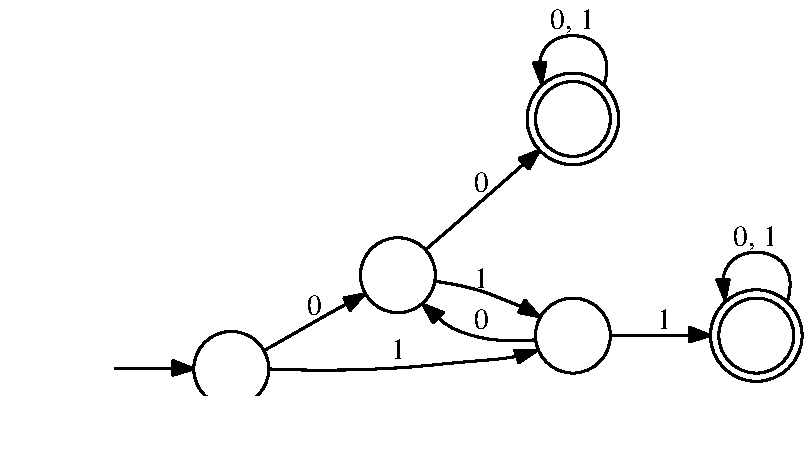
\includegraphics[scale=0.7]{consec-two.pdf}
\end{center}
\end{figure}

Give a one-sentence description of the language recognized by the DFA.
Write a regular expression for this language.

\item
Consider the following languages over the alphabet
$\Sigma = \{0, 1\}$.
\begin{itemize}
\item $L_1$: All strings that contain at least two 0s
\item $L_2$: All strings that contain at least one 1
\item $L_3$:
All strings that contain at least two 0s and at least one 1
\item $L_4$: All strings that contain at most one 0 or no 1s
\end{itemize}
Give DFAs for each of the languages $L_1$, $L_2$, $L_3$, and $L_4$.

{\bf Aside}: This example illustrates that the regular languages are
closed under intersection and complementation. Note that
$L_3 = L_1 \cap L_2$ and $L_4 = \Sigma^{*} - L_3$, where $\Sigma^{*}$
represents the language containing all strings over the alphabet
$\Sigma$.

\item
Let $E_{3}$ be the language over the alphabet
$\Sigma = \{a_{1}, a_{2}, a_{3}\}$ defined as follows.
\begin{center}
$E_{3}$: All strings in which $a_{i}$ occurs an even number of times
for some $i \in \{1, 2, 3\}$
\end{center}
Give a non-deterministic finite automaton (NFA) for the language
$E_{3}$.

\item
Write regular expressions for the following languages over the
alphabet $\Sigma = \{0, 1\}$:
\begin{enumerate}
\item All strings that contain at least one 0 and at least one 1 and
that also end with at least two 1s.
\item All strings that do not begin with 01.
\item All strings that contain an odd number of 1s.
\end{enumerate}

\item
Give a DFA for each of the following languages over the alphabet
$\Sigma = \{0, 1\}$.
\begin{enumerate}
\item The language of the following NFA.
\begin{figure}[htb]
\begin{center}
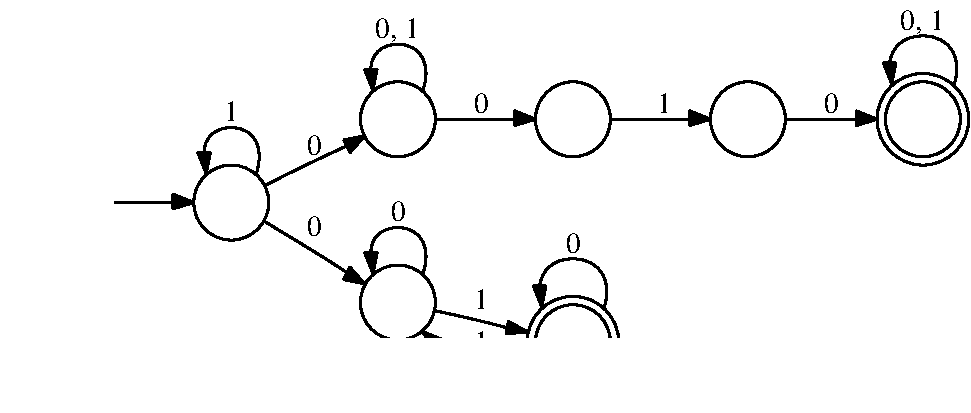
\includegraphics[scale=0.7]{substr-odd.pdf}
\end{center}
\end{figure}

\item The language of the regular expression $(0 + 01)^{*}1^{*}$.
\end{enumerate}

\item
Consider the string
\begin{verbatim}
aaabaabbababbb
\end{verbatim}
and its tokenization
\begin{verbatim}
aa a b aabb a b a bbb
\end{verbatim}

Give a flex specification with the minimum number of rules that
produces this tokenization.  Each flex rule should be as simple as
possible as well.  You may not use regular expression union (i.e.,
$R_1 + R_2$) in your solution.  Do not give any actions; just assume
that the rule returns the string that it matches.

\end{enumerate}

\end{document}
